\begin{figure}[t]
\centering
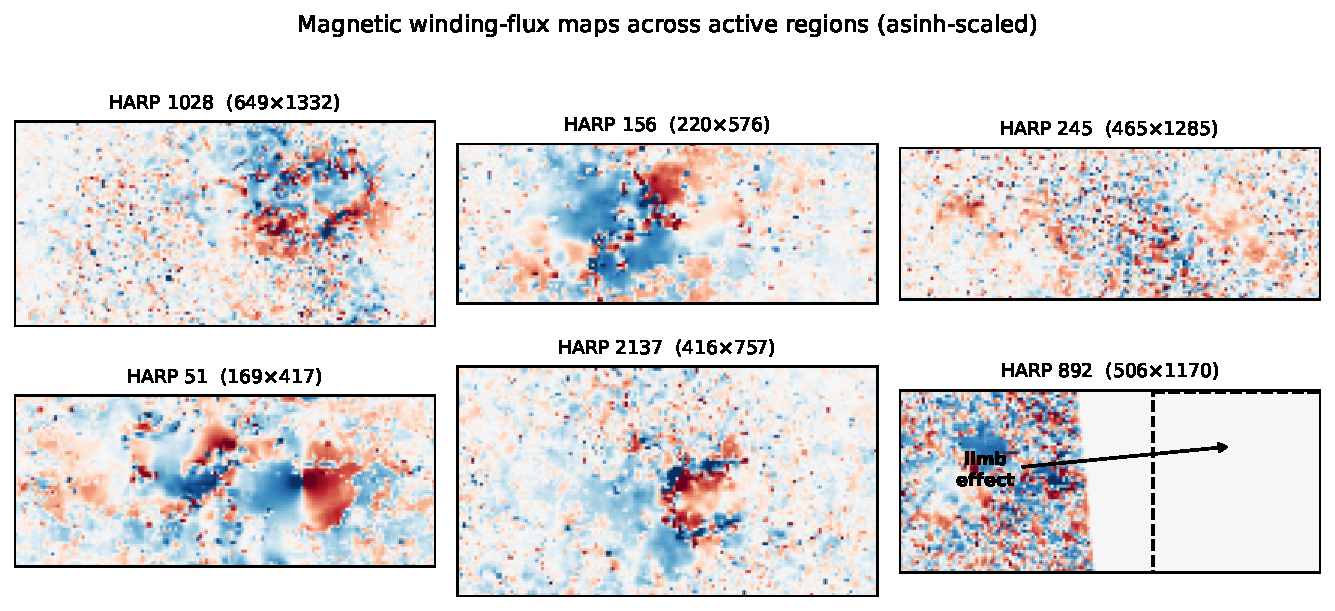
\includegraphics[width=\textwidth]{figures/fig_ar_gallery.pdf}
\caption[Active-region gallery]{\textbf{Magnetic winding-flux maps across the
active-region corpus.} One representative frame from each of six HARP regions,
asinh-scaled, with grid dimensions given. The regions differ markedly in size and
in the morphology of their signed (red/blue) winding structure, which is why the
model is evaluated leave-one-active-region-out.}
\label{fig:gallery}
\end{figure}
